\documentclass[tikz,border=9pt]{standalone}
\usepackage{amsmath,amssymb}
\usetikzlibrary{arrows.meta,positioning,calc}
\begin{document}
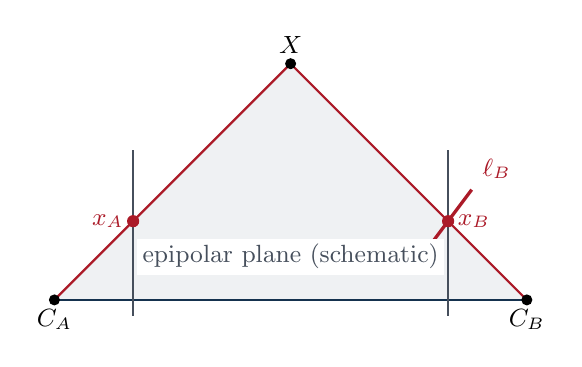
\begin{tikzpicture}[font=\small,arr/.style={-{Stealth},thick},box/.style={draw=blue!55!black,rounded corners,fill=blue!4,align=center,text width=2.9cm,minimum height=1.05cm}]
\definecolor{navy}{RGB}{21,50,78}\definecolor{solveRed}{RGB}{171,26,40}\definecolor{muted}{RGB}{70,79,92}

\coordinate (CA) at (0,0); \coordinate (CB) at (6,0); \coordinate (X) at (3,3);
\fill[navy!7] (CA)--(CB)--(X)--cycle;
\draw[navy,thick] (CA)--(CB); \draw[solveRed,thick] (CA)--(X)--(CB);
\draw[muted,thick] (1,-.2)--(1,1.9); \draw[muted,thick] (5,-.2)--(5,1.9);
\coordinate (a) at (1,1); \coordinate (b) at (5,1);
\fill (CA) circle (2pt) node[below]{$C_A$}; \fill (CB) circle (2pt) node[below]{$C_B$};
\fill (X) circle (2pt) node[above]{$X$};
\fill[solveRed] (a) circle (2.2pt) node[left]{$x_A$};
\fill[solveRed] (b) circle (2.2pt) node[right]{$x_B$};
\draw[solveRed,very thick] (4.7,.6)--(5.3,1.4) node[above right]{$\ell_B$};
\node[muted,fill=white,inner sep=2pt] at (3,.55){epipolar plane (schematic)};

\end{tikzpicture}
\end{document}
